\documentclass[xcolor=table]{beamer}
\usepackage[utf8]{inputenc}
\usepackage[english]{babel}
\usepackage{amsmath,mathrsfs,mathtext}
\usepackage{amsfonts, amssymb}
\usepackage{graphicx, epsfig}
\usepackage{subfig}

\newcommand{\hdir}{.}

\newcommand{\bz}{\mathbf{z}}
\newcommand{\bx}{\mathbf{x}}
\newcommand{\by}{\mathbf{y}}
\newcommand{\bw}{\mathbf{w}}
\newcommand{\bZ}{\mathbf{Z}}
\newcommand{\bX}{\mathbf{X}}
\newcommand{\btheta}{\boldsymbol{\theta}}
\newcommand{\bmu}{\boldsymbol{\mu}}
\newcommand{\blambda}{\boldsymbol{\lambda}}
\newcommand{\bPsi}{\boldsymbol{\Psi}}
\newcommand{\bpsi}{\boldsymbol{\psi}}
\newcommand{\bchi}{\boldsymbol{\chi}}
\newcommand{\bzeta}{\boldsymbol{\zeta}}

\usepackage{tikz}
\usepackage{color}
\usetikzlibrary{arrows,shapes,positioning,shadows,trees}

\tikzset{
  basic/.style   = {draw, drop shadow, font=\sffamily, rectangle},
  bascirc/.style = {draw, drop shadow, font=\sffamily, circle},
  root/.style    = {basic, rounded corners=2pt, thin, align=center, fill=yellow!30},
  level 2/.style = {basic, rounded corners=2pt, thin, align=center, fill=yellow!30},
  level 3/.style = {thin, align=center, text width=3.5em},
  inputs/.style  = {basic, rounded corners=5pt, thin, align=center, fill=blue!30, text width=2em},
  input/.style  = {basic, rounded corners=0pt, thin, align=center, fill=blue!30, text width=2em},
  batch/.style  = {basic, rounded corners=0pt, thin, align=center, fill=red!30, text width=2em},
  lstm/.style  = {basic, rounded corners=0pt, thin, align=center, fill=pink!30, text width=2em},
  dense/.style  = {basic, rounded corners=0pt, thin, align=center, fill=yellow!30, text width=2em},
  gate/.style  = {basic, rounded corners=5pt, thin, align=center, fill=blue!30, text width=10em},
  iofgate/.style  = {basic, rounded corners=5pt, thin, align=center, fill=red!30, text width=10em},
  memory/.style  = {basic, rounded corners=5pt, thin, align=center, fill=blue!100, text width=10em},
  iof/.style  = {basic, rounded corners=5pt, thin, align=center, fill=blue!100, text width=10em},
  gates/.style  = {basic, rounded corners=5pt, thin, align=center, fill=blue!100, text width=10em},
  memotytikz/.style  = {basic, rounded corners=5pt, thin, align=center, fill=blue!100, text width=10em},
  back/.style  = {basic, rounded corners=5pt, thin, align=center, fill=blue!100, text width=10em},
  sharing/.style   = {basic, rounded corners=5pt, thin, align=center, fill=pink!30, text width=2em},
  task/.style    = {basic, rounded corners=5pt, thin, align=center, fill=red!30, text width=2em}
}

\usetheme{Warsaw}%{Darmstadt}%{Warsaw}%{Singapore}
\usecolortheme{sidebartab}
% \definecolor{beamer@blendedblue}{RGB}{17,74,131}
\definecolor{beamer@blendedblue}{RGB}{37,39,136}
%----------------------------------------------------------------------------------------------------------
\title[\hbox to 56mm{Composition of neural networks  \hfill\insertframenumber\,/\,\inserttotalframenumber}]
{Multi-layer Neural Networks \\ for Time Series Forecast}
\author[M. Vladimirova]{\large \\Maria Vladimirova}
\institute{\footnotesize{
Moscow Institute of Physics and Technology
\vspace{0.3cm} \\
    Supervisor:  Vadim\,Strijov}}


\date{\footnotesize{MIPT, 2016}}
%----------------------------------------------------------------------------------------------------------
\begin{document}
%----------------------------------------------------------------------------------------------------------
\begin{frame}
\titlepage
\end{frame}
%----------------------------------------------------------------------------------------------------------
\begin{frame}{Multi-scale massive time series forecasting problem}
	
	\begin{block}{Goal}
		%Целью является предложить алгоритм предсказания потребления энергии для использующихся многомасштабных временных рядов.

		Building an adequate model to forecast energy consumption for using multi-scale forecasting time series.
	\end{block}

	\begin{block}{Model}
		% Предложенная модель --- это композиция нейронных сетей.
		Composition of neural networks.
	\end{block}

	\begin{block}{Solution}

		To improve the forecast quality we propose the multitask model of neural networks. 
		%Bagging of neural networks multitask model to improve the prediction quality. 
	\end{block}

\end{frame}
%----------------------------------------------------------------------------------------------------------
\begin{frame}{State of the art and problem solutions}

	\begin{itemize}
			% \item \textbf{Computer modeling of 3D structure.} \\
			\item{\footnotesize P. Cortez, M. Rio, M. Rocha, and P. Sousa, ``Multi-scale internet traffic forecasting using neural networks and time series methods'', 2012.}
			
			% \item \textbf{Quantitative structure–activity relationship (QSAR) modeling.} \\
			\item{\footnotesize K. Cho, B. Merrienboer, F. Bougares, H. Schwenk, and Y. Bengio, ``Learning phrase representations using RNN encoder-decoder for statistical machine translation'', 2014.} 
				 
			%  \textbf{The use of neural networks for researching problems.} \\
			\item{\footnotesize Z. Cui, W. Chen, and Y. Chen, ``Multi-scale convolutional neural networks for time series classification'', 2016. }
				
	\end{itemize}

\end{frame}
%----------------------------------------------------------------------------------------------------------
\begin{frame}{\textit{Energy-Weather, Multi-scale Time Series in Warsaw}}


	\vspace{-0.1cm}
	Dataset from {\footnotesize http://gdudek.el.pcz.pl/varia/stlf-dat}



	\begin{itemize}
		\item contains electricity load time series, weather time series (temperature, precipitation, wind force, humidity, solar), holiday schedule;
		\item energy consumption was measured hourly from 1999 to 2004, 52512 observations;
		\item weather was measured daily, 2188 observations.
		
	\end{itemize}

	\vspace{-0.3cm}
	\begin{figure}
		\includegraphics[width=1\linewidth]{\hdir/electricity.png}
		% \caption{Electic load data}
	\end{figure}
	\vspace{-0.5cm}
	\center{Figure: Electic load data}
\end{frame}
%----------------------------------------------------------------------------------------------------------
\begin{frame}{Problem statement}

%Now, let’s state formally our problem. We have a design matrix, which consists of N proteins description 
	\begin{block}{The given set}
	 	Sample set: $\mathfrak{D} = \{(\bx_i, y_i)\}_{i = 1}^m$, where $\bx_i \in \mathbb{R}^{n}$~-- independed variable, $y_i\in \mathbb{R}^{1}$~--~target value, $m = 24,\ n = 2188$.
	\end{block}

	\begin{block}{Assume}
		Output	vector $y_i = f(\bw, \bx_i) + \varepsilon(\bx_i)$, where $\varepsilon_i = \varepsilon(\bx_i)$~-- random variable, $\bw$~-- vector of parameters, $f: (\bw, \bx_i) \mapsto y_i$~-- regression model.
	\end{block}

	\begin{block}{Find}
    	Regression function $f(\hat{\bw}, \bx)$, where $\hat{\bw} = \mathop{\text{argmin}} \limits_{\bw \in \mathbb{R}^{m}} S[\bw | f(\bw, \bx), y]$~-- optimal parameters, $S$~-- loss function  
    	\[
    		S = sMAPE = \sum_{i=1}^m \frac{2 |\varepsilon(\bx_i)|}{y_i + f(\bw, \bx_i)}.
    	\]
  	\end{block}
\end{frame}
%----------------------------------------------------------------------------------------------------------
\begin{frame}{Composition of neural networks}

	% $\bx \longrightarrow \text{Batch} \longrightarrow \text{LSTM} \longrightarrow \text{LSTM} \longrightarrow \text{Dense} \longrightarrow y$

	\hspace*{-0.5cm}
	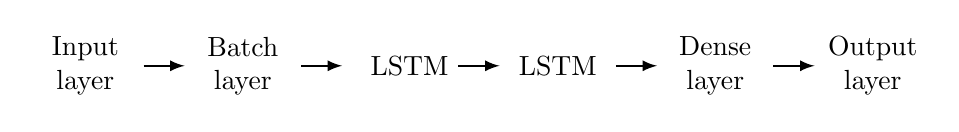
\begin{tikzpicture}[node distance=2cm,
		  circle/.style={sibling distance=17mm},
		  edge from parent/.style={-,draw}, 
		  >=latex]



		\node[level 3] (i0) {Input\\ layer};

		\node[level 3, right of = i0] (b0) {Batch\\ layer};

		\node[level 3, right of = b0] (l0) {\ \ LSTM};

		\node[level 3, right of = l0] (l2) {LSTM};

		\node[level 3, right of = l2] (d0) {Dense\\ layer};

		\node[level 3, right of = d0] (o0) {Output\\ layer};

		
		\path[->, thick] 	(i0) edge node{} (b0)
			
					(b0) edge node{} (l0)
	
					(l0) edge node{} (l2)
		
					(l2) edge node{} (d0)

					(d0) edge node{} (o0);

	\end{tikzpicture}

	\begin{itemize}
		\item {\bf Input layer}: the set of input units $\bx$. 
		\item {\bf Batch layer}: the normalization of activations that depends on the mini-batch, allows efficient training.
		\item {\bf Long Short-Time Memory (LSTM) layer}: a recurrent neural network (RNN) architecture that is designed to be better at storing and accessing information than standard RNNs.
		\item {\bf Dense layer}: a fully connected layer with reverse normalization.
		\item {\bf Output layer}: a layer with predicted target values $y$. 

	\end{itemize}


	
 


	% \pgfdeclarelayer{background}
	% \pgfdeclarelayer{foreground}
	% \pgfsetlayers{background,main,foreground}
	% \hspace*{-4cm}
	% \begin{tikzpicture}[node distance=2cm,
	% 	  circle/.style={sibling distance=17mm},
	% 	  edge from parent/.style={-,draw}, 
	% 	  >=latex]



	% 	\node[input] (i0) {\ \\ \ \\ \ \\ \ \\ \ \\ };
	% 	\node[level 3, below of = i0] (i1) {Input\\ layer};

	% 	\node[batch, right of = i0] (b0) {\ \\ \ \\ \ \\ \ \\ \ \\ \ \\ \ \\};
	% 	\node[level 3, below of = b0] (b1) {\ \\ Batch\\ normalization};

	% 	\node[lstm, right of = b0] (l0) {\ \\ \ \\ \ \\ \ \\ \ \\ \ \\};
	% 	\node[level 3, below of = l0] (l1) {LSTM};

	% 	\node[lstm, right of = l0] (l2) {\ \\ \ \\ \ \\ \ \\ \ \\ \ \\};
	% 	\node[level 3, below of = l2] (l3) {LSTM};

	% 	\node[dense, right of = l2] (d0) {\ \\ \ \\ \ \\ \ \\ \ \\ \ \\};
	% 	\node[level 3, below of = d0] (d1) {Dense\\ layer};

	% 	\node[input, right of = d0] (o0) {\ \\ \ \\ \ \\ \ \\};
	% 	\node[level 3, below of = o0] (o1) {Output\\ layer};
		
	% 	\path[->] 	(i0) edge node{} (b0)
			
	% 				(b0) edge node{} (l0)
	
	% 				(l0) edge node{} (l2)
		
	% 				(l2) edge node{} (d0)

	% 				(d0) edge node{} (o0);

	% \end{tikzpicture}
 


\end{frame}
%----------------------------------------------------------------------------------------------------------
\begin{frame}{Batch-normalization: faster learning and higher overall accuracy}
	
	% Рассмотрим классическую нейронную сеть с несколькими слоями. Каждый слой имеет множество входов и множество выходов. Сеть обучается методом обратного распространения ошибки, по батчам, то есть ошибка считается по какому-то подмножестве обучающей выборки.

	% Стандартный способ нормировки — для каждого k рассмотрим распределение элементов батча. Вычтем среднее и поделим на дисперсию выборки, получив распределение с центром в 0 и дисперсией 1. Такое распределение позволит сети быстрее обучатся, т.к. все числа получатся одного порядка. Но ещё лучше ввести две переменные для каждого признака, обобщив нормализацию следующим образом:


	% Получим среднее и дисперсию. Эти параметры будут входить в алгоритм обратного распространения ошибки. Тем самым получаем batch normalization слой с 2*k параметрами, который и будем добавлять в архитектуру предложенной сети


	%Training Deep Neural Networks is complicated by the fact that the distribution of each layer’s inputs changes during training as the parameters of the previous layers change. This slows down the training by requiring lower learning rates and careful parameter initialization, and makes it hard to train models with saturating nonlinearities. 
	% \vspace{-0.3cm}
	%  \begin{figure}[!h]
 %   	 	\center{\includegraphics[width=0.7\linewidth]{\hdir/batch.png}}
	%  \end{figure}
	\vspace{-0.3cm}
	\begin{block}{Mini-batch is a subpart of the training set $\mathcal{B} = \{x_1, \dots, x_\ell\}$}
		\footnotesize{
		\begin{itemize}
			\item the gradient of the loss over a mini-batch is an estimate of the gradient over the training set, whose quality improves as the batch size increases,
			\item computation over a batch is more efficient than $\ell$ computations for individual examples.
		\end{itemize}}
		% Using mini-batches is helpful: first, the gradient of the loss over a mini-batch is an estimate of the gradient over the training set, whose quality improves as the batch size increases; second, computation over a batch can be much more efficient than $\ell$ computations for individual examples, due to the parallelism afforded by the modern computing platforms.
	\end{block}

	\vspace{-0.7cm}
	\begin{align*}
		\mu_{\mathcal{B}} &\leftarrow \frac{1}{\ell} \sum_{i = 1}^\ell x_i; &\qquad \text{mini-batch mean};\\
		\sigma^2_{\mathcal{B}} &\leftarrow \frac{1}{\ell} \sum_{i = 1}^\ell (x_i - \mu_{\mathcal{B}})^2&\qquad \text{mini-batch variance};\\
		\hat{x}_i &\leftarrow \frac{x_i - \mu_{\mathcal{B}}}{\sqrt{\sigma^2_{\mathcal{B}} + \epsilon}} &\qquad \text{normalize}.
		% \intertext{Reverse normalization:}
		% y_i &\leftarrow \gamma \hat{x}_i + \beta \equiv BN_{\gamma, \beta}(x_i) &\qquad \text{scale and shift}.
	\end{align*}

	\vspace{-0.1cm}
	Reverse normalization: $y_i \leftarrow \gamma \tilde{x}_i + \beta \equiv BN_{\gamma, \beta}(x_i), \text{where} \ \gamma,\ \beta$ are parameters to be learned. 


	% \vspace{-0.2cm}
	% \begin{itemize}
	% 	\item allows us to use much higher learning rates and be less careful about initialization;
	% 	\vspace{-0.1cm}
	% 	\item acts as a regularizer.	
	% \end{itemize}

 	\vspace{-0.1cm}
	{\footnotesize Ioffe S., Szegedy C. ``Batch Normalization'', 2015}
\end{frame}
%----------------------------------------------------------------------------------------------------------
\begin{frame}{Recurrent Neural Network}
	% https://habrahabr.ru/company/dca/blog/274027/

	% Основное отличие рекурентных сетей (Recurrent Neural Network, RNN) от традиционных заключается в логике работы сети, при которой каждый нейрон взаимодействует сам с собой. На вход таким сетям как правило передаётся сигнал, являющийся некоторой последовательностью. Каждый элемент такой последовательности поочерёдно передаётся одним и тем же нейронам, которые своё же предсказание возвращают себе вместе со следующим её элементом, до тех пор пока последовательность не закончится. Такие сети, как правило, используются при работе с последовательной информацией. Элементы рекурентной сети изображают как обычные нейроны с дополнительной циклической стрелкой, которая демонстрирует то, что кроме входного сигнала нейрон использует также своё дополнительное скрытое состояние. Если «развернуть» такое изображение, получится целая цепочка одинаковых нейронов, каждый из которых получает на вход свой элемент последовательности, выдаёт предсказание и передаёт его дальше по цепочке как своего рода ячейку памяти. Нужно понимать, что это абстракция, поскольку это один и тот же нейрон, который отрабатывает несколько раз подряд. 
	
	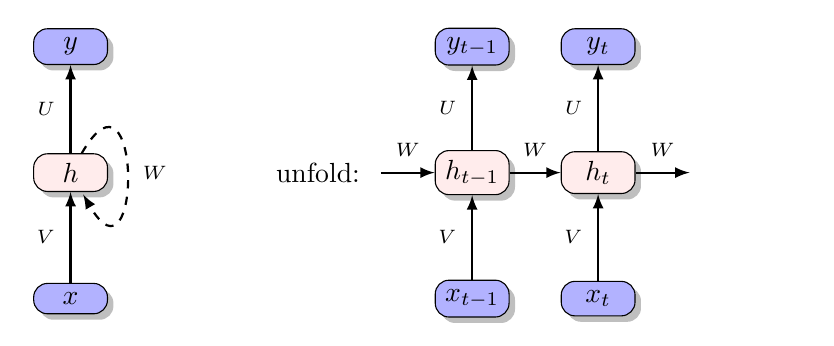
\begin{tikzpicture}[node distance=1.6cm,
		  circle/.style={sibling distance=22mm},
		  edge from parent/.style={-,draw}, 
		  >=latex]

		% freeforward NN, level 1
		\node[inputs] (i1) {$x$};
		\node[sharing, above of = i1] (i2) {$h$};
		\node[inputs, above of = i2] (i3) {$y$};

		\node[level 3, right of = i2] (u0) {};

		\node[level 3, right of = u0] (u1) {unfold:\ \ \ };

		% RNN
		\node[sharing, right of = u1, node distance=1.9cm] (r1) {$h_{t-1}$};
		\node[inputs, below of = r1] (r0) {$x_{t-1}$};
		\node[inputs, above of = r1] (r2) {$y_{t-1}$};

		\node[sharing, right of = r1] (t1) {$h_{t}$};
		\node[inputs, below of = t1] (t0) {$x_{t}$};
		\node[inputs, above of = t1] (t2) {$y_{t}$};
		\node[level 3, right of = t1, node distance=1.9cm] (u2) {};



		\path[->, thick]	(i1) edge node [left=0.07,swap] {$\substack{V}$} (i2)
					(i2) edge node [left=0.07,swap] {$\substack{U}$} (i3)
					(i2) edge [out=60,in=-60, loop, dashed] node [right=0.07,swap] {$\substack{W}$} (i2)

					(r0) edge node [left=0.07,swap] {$\substack{V}$} (r1)
					(r1) edge node [left=0.07,swap] {$\substack{U}$} (r2)
					(t0) edge node [left=0.07,swap] {$\substack{V}$} (t1)
					(t1) edge node [left=0.07,swap] {$\substack{U}$} (t2)
					(r1) edge node [above=0.07,swap] {$\substack{W}$} (t1)
					(u1) edge node [above=0.07,swap] {$\substack{W}$} (r1)
					(t1) edge [out=0, in=180] node [above=0.07,swap] {$\substack{W}$} (u2);
	\end{tikzpicture}


	
	$$	\qquad h_t = g(V x_t + W h_{t-1} + b_h),$$
	$$	\qquad y_t = f(U h_t + b_y).$$
	
\end{frame}


%----------------------------------------------------------------------------------------------------------
\begin{frame}{Backpropagation Through Time}
	% https://habrahabr.ru/company/dca/blog/274027/

	% Основное отличие рекурентных сетей (Recurrent Neural Network, RNN) от традиционных заключается в логике работы сети, при которой каждый нейрон взаимодействует сам с собой. На вход таким сетям как правило передаётся сигнал, являющийся некоторой последовательностью. Каждый элемент такой последовательности поочерёдно передаётся одним и тем же нейронам, которые своё же предсказание возвращают себе вместе со следующим её элементом, до тех пор пока последовательность не закончится. Такие сети, как правило, используются при работе с последовательной информацией. Элементы рекурентной сети изображают как обычные нейроны с дополнительной циклической стрелкой, которая демонстрирует то, что кроме входного сигнала нейрон использует также своё дополнительное скрытое состояние. Если «развернуть» такое изображение, получится целая цепочка одинаковых нейронов, каждый из которых получает на вход свой элемент последовательности, выдаёт предсказание и передаёт его дальше по цепочке как своего рода ячейку памяти. Нужно понимать, что это абстракция, поскольку это один и тот же нейрон, который отрабатывает несколько раз подряд. 
	\begin{columns}[c]

	\column{0.38\textwidth}
	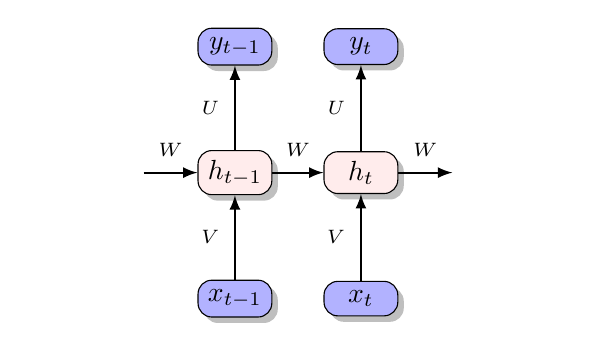
\begin{tikzpicture}[node distance=1.6cm,
		  circle/.style={sibling distance=22mm},
		  edge from parent/.style={-,draw}, 
		  >=latex]


		\node[level 3] (u1) {\ \ \ };

		% RNN
		\node[sharing, right of = u1, node distance=1.9cm] (r1) {$h_{t-1}$};
		\node[inputs, below of = r1] (r0) {$x_{t-1}$};
		\node[inputs, above of = r1] (r2) {$y_{t-1}$};

		\node[sharing, right of = r1] (t1) {$h_{t}$};
		\node[inputs, below of = t1] (t0) {$x_{t}$};
		\node[inputs, above of = t1] (t2) {$y_{t}$};
		\node[level 3, right of = t1, node distance=1.9cm] (u2) {};



		\path[->, thick]	
					(r0) edge node [left=0.07,swap] {$\substack{V}$} (r1)
					(r1) edge node [left=0.07,swap] {$\substack{U}$} (r2)
					(t0) edge node [left=0.07,swap] {$\substack{V}$} (t1)
					(t1) edge node [left=0.07,swap] {$\substack{U}$} (t2)
					(r1) edge node [above=0.07,swap] {$\substack{W}$} (t1)
					(u1) edge node [above=0.07,swap] {$\substack{W}$} (r1)
					(t1) edge [out=0, in=180] node [above=0.07,swap] {$\substack{W}$} (u2);
	\end{tikzpicture}


	\column{0.62\textwidth}
	$$	\qquad h_t = g(V x_t + W h_{t-1} + b_h),$$
	$$	\qquad y_t = f(U h_t + b_y).$$

	\center{Loss function:}
	\[
		S(y, a) = \sum_{t = 1}^T S_t(y_t, a_t)
	\]

	\end{columns}


	\vspace{1cm}
	\[
		\frac{\partial S_\tau}{\partial h_t} = \frac{\partial S_\tau}{\partial h_\tau} \prod_{k = t}^{T-1} \frac{\partial h_{k+1}}{\partial h_k} = \frac{\partial S_\tau}{\partial h_\tau} \prod_{k = t}^{T-1} \underbrace{diag\left(g'(\dots)\right)W}_{\substack{exploding\\ or\ vanishing\\gradients}}
	\]
	
\end{frame}
%----------------------------------------------------------------------------------------------------------
\begin{frame}{Long Short Term Memory}

	\begin{columns}[c]
    \column{0.38\textwidth}
	
 
		\vspace{-0.3cm}
			\hspace*{-0.5cm}
	   	 	\includegraphics[width=1.3\textwidth]{\hdir/lstm_nice.png}

	 	 	
	\column{0.62\textwidth}
		% \begin{tikzpicture}[node distance=1cm,
		%   circle/.style={sibling distance=17mm},
		%   edge from parent/.style={-,draw}, 
		%   >=latex]
		
		% 	\node[gate] (i0) {gate values in $[0,1]$};
		% 	\node[iofgate, below of = i0] (i1) {$i_t, o_t, f_t$~-- input, output, forget gates};
		% 	\node[memory, below of = i1] (i2) {$c_t$~-- memory};
		% \end{tikzpicture}
		% \center{gate values in $[0,1]$}\\
		% \center{$i_t, o_t, f_t$~-- input, output, forget gates}\\
		% \center{$c_t$~-- memory}
		% \vspace{-0.1cm}
		\ Input gate: 
		\vspace{-0.3cm}
		\begin{equation}
		\nonumber
			i_t = \sigma(W_{xi} x_t + W_{hi} h_t + W_{ci} c_{t-1} + b_i)
	 	\end{equation}
	 	\vspace{-0.1cm}
	 	Forget gate:
	 	\vspace{-0.3cm}
	 	\begin{equation}
	 	\nonumber
			f_t = \sigma(W_{xf} x_t + W_{hf} h_t + W_{cf} c_{t-1} + b_f)
	 	\end{equation}
	 	\vspace{-0.1cm}
	 	Memory:
	 	\vspace{-0.3cm}
	 	\begin{equation}
	 	 \nonumber
			\ c_t = f_t c_{t-1} + i_t \tanh(W_{xc} x_t + W_{hc} h_{t-1} + b_c)
	 	\end{equation}
	 	\vspace{-0.1cm}
	 	Output gate:
	 	\vspace{-0.3cm}
	 	\begin{equation}
	 	\nonumber
			\ o_t = \sigma(W_{xo} x_t + W_{ho} h_{t-1} + W_{c0} c_{t} + b_o)
	 	\end{equation}
	 	\vspace{-0.2cm}
	 	Gate values in $[0,1]$.
	
	 	\begin{equation}
	 	\nonumber
			h_t = o_t \tanh(c_t)
	 	\end{equation}

	\end{columns}
	
	% \vspace{-0.1cm}
	% After batch-normalization:
	% \vspace{-0.6cm}
	% \begin{equation}

	% 	i_t = \sigma(W_{xi} x_t + W_{hi} h_t + W_{ci} c_{t-1} + b_i)
 % 	\end{equation}
 % 	\begin{equation}
	% 	f_t = \sigma(W_{xf} x_t + W_{hf} h_t + W_{cf} c_{t-1} + b_f)
 % 	\end{equation}
 % 	 \begin{equation}
	% 	c_t = f_t c_{t-1} + i_t \tanh(W_{xc} x_t + W_{hc} h_{t-1} + b_c)
 % 	\end{equation}
 % 	\begin{equation}
	% 	o_t = \sigma(W_{xo} x_t + W_{ho} h_{t-1} + W_{c0} c_{t} + b_o)
 % 	\end{equation}
 % 	\begin{equation}
	% 	h_t = o_t \tanh(c_t)
 % 	\end{equation}

 \vspace{0.2cm}
 {\footnotesize Graves, Alex: “Generating sequences with recurrent neural networks”, 2014}

\end{frame}
%----------------------------------------------------------------------------------------------------------
\begin{frame}{Computational Experiment}
	
\hspace*{-0.5cm}
	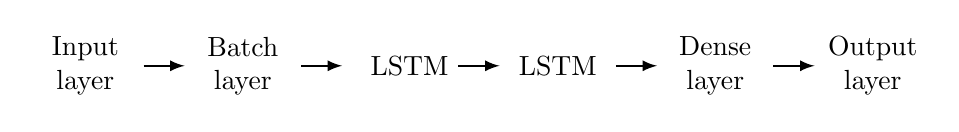
\begin{tikzpicture}[node distance=2cm,
		  circle/.style={sibling distance=17mm},
		  edge from parent/.style={-,draw}, 
		  >=latex]



		\node[level 3] (i0) {Input\\ layer};

		\node[level 3, right of = i0] (b0) {Batch\\ layer};

		\node[level 3, right of = b0] (l0) {\ \ LSTM};

		\node[level 3, right of = l0] (l2) {LSTM};

		\node[level 3, right of = l2] (d0) {Dense\\ layer};

		\node[level 3, right of = d0] (o0) {Output\\ layer};

		
		\path[->, thick] 	(i0) edge node{} (b0)
			
					(b0) edge node{} (l0)
	
					(l0) edge node{} (l2)
		
					(l2) edge node{} (d0)

					(d0) edge node{} (o0);

	\end{tikzpicture}



	\begin{itemize}
		\item {\bf Input layer}: $\bx\ 1 \times 2188$ (90 days). 
		\item {\bf Batch layer}: mini-batch of the size 240 (10 days), $\text{batch-size} = k$, getting average value and variance.
		\item {\bf LSTM layer}: input design matrix shape $240\times k$, output matrix shape $50 \times k$.
		\item {\bf Dense layer}: a fully connected layer, $k$ output units.
		\item {\bf Output layer}: reverse normalization: multiply by variance, add up to average value, predicted values $\by$ with $k$ predicted observations. 
	\end{itemize}

\end{frame}
%----------------------------------------------------------------------------------------------------------
\begin{frame}{Results}
	 
	\hspace*{-1.1cm}
	\vspace*{0cm}
	 	\centering
   	 	\includegraphics[width=0.4\textwidth]{\hdir/oneday.png}
   	 	\hspace*{-0.2cm}
   	 	\includegraphics[width=0.4\textwidth]{\hdir/twodays.png}
   	 	\hspace*{-0.2cm}
   	 	\includegraphics[width=0.4\textwidth]{\hdir/fivedays.png}

   	\hspace*{-1.1cm}
   	\vspace{1cm}
   	 	\centering
   	 	\includegraphics[width=0.4\textwidth]{\hdir/tendays.png}
   	 	\hspace*{-0.2cm}
   	 	\includegraphics[width=0.405\textwidth]{\hdir/twentydays.png}
   	 	\hspace*{-0.2cm}
   	 	\includegraphics[width=0.42\textwidth]{\hdir/month.png}


\end{frame}
%----------------------------------------------------------------------------------------------------------
\begin{frame}{Forecast}
	\begin{figure}[!h]
   	 	\center{\includegraphics[width=0.8\linewidth]{\hdir/badforecast.png}}
	 \end{figure}
	
	Good at making short-term forecasts ($\sim$10 days), but long-term forecast can go to infinity.

\end{frame}
%----------------------------------------------------------------------------------------------------------
\begin{frame}{Comparison of results}
\footnotesize{
\begin{table}[]
\centering
\label{my-label}
\begin{tabular}{llllll}
                                                                &                       & \multicolumn{4}{l}{\textbf{Composition of Neural Networks}}                                                                                                                                                                           \\ \cline{3-6} 
                                                                & \multicolumn{1}{l|}{} & \multicolumn{1}{l|}{\cellcolor[HTML]{ECF4FF}MAE, train} & \multicolumn{1}{l|}{\cellcolor[HTML]{ECF4FF}MAPE, train} & \multicolumn{1}{l|}{\cellcolor[HTML]{ECF4FF}MAE, test} & \multicolumn{1}{l|}{\cellcolor[HTML]{ECF4FF}MAPE, test} \\ \cline{1-1} \cline{3-6} 
\multicolumn{1}{|l|}{\cellcolor[HTML]{ECF4FF}Energy}            & \multicolumn{1}{l|}{} & \multicolumn{1}{l|}{14445.89}                           & \multicolumn{1}{l|}{0.045855}                            & \multicolumn{1}{l|}{22422.82}                          & \multicolumn{1}{l|}{0.074466}                           \\ \cline{1-1}
\multicolumn{1}{|l|}{\cellcolor[HTML]{ECF4FF}Max Temperature}   & \multicolumn{1}{l|}{} & \multicolumn{1}{l|}{2.622256}                           & \multicolumn{1}{l|}{0.955615}                            & \multicolumn{1}{l|}{3.093671}                          & \multicolumn{1}{l|}{0.765553}                           \\ \cline{1-1}
\multicolumn{1}{|l|}{\cellcolor[HTML]{ECF4FF}Min Temperature}   & \multicolumn{1}{l|}{} & \multicolumn{1}{l|}{2.166025}                           & \multicolumn{1}{l|}{6.667440}                            & \multicolumn{1}{l|}{2.525723}                          & \multicolumn{1}{l|}{2.029947}                           \\ \cline{1-1}
\multicolumn{1}{|l|}{\cellcolor[HTML]{ECF4FF}Wind}              & \multicolumn{1}{l|}{} & \multicolumn{1}{l|}{0.851419}                           & \multicolumn{1}{l|}{0.302157}                            & \multicolumn{1}{l|}{0.897353}                          & \multicolumn{1}{l|}{0.308688}                           \\ \cline{1-1}
\multicolumn{1}{|l|}{\cellcolor[HTML]{ECF4FF}Relative Humidity} & \multicolumn{1}{l|}{} & \multicolumn{1}{l|}{0.070334}                           & \multicolumn{1}{l|}{0.105500}                            & \multicolumn{1}{l|}{0.086160}                          & \multicolumn{1}{l|}{0.124058}                           \\ \cline{1-1}
\multicolumn{1}{|l|}{\cellcolor[HTML]{ECF4FF}Solar}             & \multicolumn{1}{l|}{} & \multicolumn{1}{l|}{3.010862}                           & \multicolumn{1}{l|}{0.577961}                            & \multicolumn{1}{l|}{4.128087}                          & \multicolumn{1}{l|}{0.725591}                           \\ \cline{1-1} \cline{3-6} 
                                                                &                       &                                                         &                                                          &                                                        &                                                         \\
                                                                &                       & \multicolumn{4}{l}{\textbf{Random Forest}}                                                                                                                                                                                            \\ \cline{3-6} 
                                                                & \multicolumn{1}{l|}{} & \multicolumn{1}{l|}{\cellcolor[HTML]{ECF4FF}MAE, train} & \multicolumn{1}{l|}{\cellcolor[HTML]{ECF4FF}MAPE, train} & \multicolumn{1}{l|}{\cellcolor[HTML]{ECF4FF}MAE, test} & \multicolumn{1}{l|}{\cellcolor[HTML]{ECF4FF}MAPE, test} \\ \cline{1-1} \cline{3-6} 
\multicolumn{1}{|l|}{\cellcolor[HTML]{ECF4FF}Energy}            & \multicolumn{1}{l|}{} & \multicolumn{1}{l|}{6211.97}                            & \multicolumn{1}{l|}{0.019912}                            & \multicolumn{1}{l|}{25113.72}                          & \multicolumn{1}{l|}{0.082950}                           \\ \cline{1-1}
\multicolumn{1}{|l|}{\cellcolor[HTML]{ECF4FF}Max Temperature}   & \multicolumn{1}{l|}{} & \multicolumn{1}{l|}{0.913400}                           & \multicolumn{1}{l|}{0.407978}                            & \multicolumn{1}{l|}{3.029345}                          & \multicolumn{1}{l|}{0.455047}                           \\ \cline{1-1}
\multicolumn{1}{|l|}{\cellcolor[HTML]{ECF4FF}Min Temperature}   & \multicolumn{1}{l|}{} & \multicolumn{1}{l|}{0.838439}                           & \multicolumn{1}{l|}{1.981043}                            & \multicolumn{1}{l|}{2.710675}                          & \multicolumn{1}{l|}{2.460068}                           \\ \cline{1-1}
\multicolumn{1}{|l|}{\cellcolor[HTML]{ECF4FF}Wind}              & \multicolumn{1}{l|}{} & \multicolumn{1}{l|}{0.337707}                           & \multicolumn{1}{l|}{0.121678}                            & \multicolumn{1}{l|}{0.897624}                          & \multicolumn{1}{l|}{0.344472}                           \\ \cline{1-1}
\multicolumn{1}{|l|}{\cellcolor[HTML]{ECF4FF}Relative Humidity} & \multicolumn{1}{l|}{} & \multicolumn{1}{l|}{0.028134}                           & \multicolumn{1}{l|}{0.041241}                            & \multicolumn{1}{l|}{0.082655}                          & \multicolumn{1}{l|}{0.114359}                           \\ \cline{1-1}
\multicolumn{1}{|l|}{\cellcolor[HTML]{ECF4FF}Solar}             & \multicolumn{1}{l|}{} & \multicolumn{1}{l|}{1.212832}                           & \multicolumn{1}{l|}{0.253059}                            & \multicolumn{1}{l|}{4.294036}                          & \multicolumn{1}{l|}{0.811916}                           \\ \cline{1-1} \cline{3-6} 
\end{tabular}
\end{table}}
\end{frame}
%----------------------------------------------------------------------------------------------------------
% \begin{frame}{Forecast}
		
	% TODO picture
	
%  	\pgfdeclarelayer{background}
% 	\pgfdeclarelayer{foreground}
% 	\pgfsetlayers{background,main,foreground}
% 	\begin{tikzpicture}[node distance=2cm,
% 		  circle/.style={sibling distance=17mm},
% 		  edge from parent/.style={-,draw}, 
% 		  >=latex]

% 		% root of the the initial tree, level 1
% 		\node[inputs] (i1) {$x_1$};
% 		\node[inputs, right of = i1] (i2) {$x_2$};
% 		\node[right of = i2] (i3) {$\dots$};
% 		\node[inputs, right of = i3] (i4) {$x_K$};
% 		\node[level 3, right of = i4] (i5) {Inputs};

% 		% shared nodes, level 2
% 		\node[sharing, below left of = i1] (s1) {$z_1$};
% 		\node[sharing, right of = s1] (s2) {$z_2$};
% 		\node[right of = s2] (s3) {$\dots$};
% 		\node[sharing, right of = s3] (s4) {$z_{H-1}$};
% 		\node[sharing, right of = s4] (s5) {$z_H$};
% 		\node[level 3, right of = s5, node distance=1.5cm] (s6) {Sharing \\nodes};

% 	    \begin{pgfonlayer}{background}
% 	      	\path (s1.west)+(-0.2,0.5) node (a) {};
% 	        \path (s5.east |- s5.south)+(0.2,-0.25) node (b) {};
	         
% 	        \path[fill=yellow!20, rounded corners, draw=black!50, dashed]
% 	            (a) rectangle (b);
%         \end{pgfonlayer}

% 		% tasks, level 3
% 		\node[task, below right of = s1] (t1) {$f_1$};
% 		\node[task, right of = t1] (t2) {$f_2$};
% 		\node[right of = t2] (t3) {$\dots$};
% 		\node[task, right of = t3] (t4) {$f_M$};
% 		\node[level 3, right of = t4] (t5) {Tasks};

% 		\path[-] 	(i1) edge node{} (s1)
% 						 edge node{} (s2)
% 						 edge node{} (s4)

% 					(i2) edge node{} (s1)
% 						 edge node{} (s2)
% 						 edge node{} (s4)

% 					(i4) edge node{} (s2)
% 						 edge node{} (s4)
% 						 edge node{} (s5)

% 					(s1) edge node{} (t1)
% 						 edge node{} (t2)
% 						 %edge node{} (t4)

% 					(s2) edge node{} (t1)
% 						 edge node{} (t2)
% 						 edge node{} (t4)

% 					(s4) edge node{} (t1)
% 						 edge node{} (t2)
% 						 edge node{} (t4)

% 					(s5) %edge node{} (t1)
% 						 edge node{} (t2)
% 						 edge node{} (t4);

% 	\end{tikzpicture}



% \end{frame}
%----------------------------------------------------------------------------------------------------------
\begin{frame}{Data correlations}
	\begin{figure}[!h]
   	 	\center{\includegraphics[width=1\linewidth]{\hdir/corr.png}}
	 \end{figure}
	\vspace{-0.5cm}
	The most correlated tasks: 0 -- 4, 6 -- 15, 21 -- 23. 

	We can use multi-task learning.

\end{frame}
%----------------------------------------------------------------------------------------------------------
% \begin{frame}{Multi-task learning: learns related problems together}
% %Multi-task learning (MTL) is an approach to machine learning that learns a problem together with other related problems at the same time, using a shared representation. This often leads to a better model for the main task, because it allows the learner to use the commonality among the tasks. 

% 	% \begin{columns}[c]
%  %    \column{0.73\textwidth}
%  	\vspace{-0.2cm}
% 	\begin{block}{Problem formulation}
% 		\begin{itemize}
% 	 		\item Probability distributions $p_1, \dots, p_m$ on $\mathbb{R}^n \times \mathbb{R}$;
% 	 		\vspace{-0.1cm}
% 	 		\item Data: $\mathbf{d} = \left((\mathbf{x}^1, y^1), \dots,(\mathbf{x}^t, y^t) \right) \sim p^t$, $t = 1,\dots,m$;
% 	 		\vspace{-0.1cm}
% 	 		\item Learn predicting models $f(\bw_1), \dots, f(\bw_m)$, such, that
% 	 			\vspace{-0.2cm}
% 	 			\[
% 	 			\begin{aligned}
% 	 				& \underset{[\bw_1,\dots,\bw_m] \in \bw}{\text{minimize}}
% 	 				& &  \dfrac{1}{m}\sum_{t=1}^m S(f(\mathbf{x}^t, \bw_t), y^t),
% 	 			\end{aligned}
% 	 			\]
% 	 		\vspace{-0.7cm}
% 	 		\item $\bw$ encourages ``common structure'' of the tasks.
% 	 	\end{itemize}
% 	\end{block}

% 	\begin{columns}[c]
%     \column{0.5\textwidth}
%     	% \hspace*{-3cm}
% 		\begin{tikzpicture}[node distance=1.3cm,
% 		  circle/.style={sibling distance=17mm},
% 		  edge from parent/.style={-,draw}, 
% 		  >=latex]


% 		\node[input] (i0) {$x$};
% 		% \node[level 3, below of = i0] (i1) {Input};


% 		\node[dense, right of = i0] (d0) {\ \\ \ \\};
% 		% \node[level 3, below of = d0] (d1) {Algorithm};

% 		\node[input, right of = d0] (o0) {$y$} ;
% 		% \node[level 3, below of = o0] (o1) {Output};

% 		\path[->] 	(i0) edge node{} (d0)

% 					(d0) edge node{} (o0);

% 	\end{tikzpicture}

% 	\ \\
% 	\ \\
% 	Single-task	model
% 	\column{0.5\textwidth}
% 	% \hspace*{-3cm}
% 	\begin{tikzpicture}[node distance=1.3cm,
% 		  circle/.style={sibling distance=17mm},
% 		  edge from parent/.style={-,draw}, 
% 		  >=latex]



% 		\node[input] (i0) {$x_1$};
% 		\node[input, below of = i0] (i1) {$\dots$};
% 		\node[input, below of = i1] (i2) {$x_t$};
% 		% \node[level 3, below of = i2] (i3) {Inputs};


% 		\node[dense, right of = i1] (d0) {\ \\ \ \\ \ \\ };
% 		\node[level 3, below of = d0] (d1) {\ \\ \ \\};
% 		% \node[level 3, below of = d1] (d2) {Algorithm};

% 		\node[input, right of = d0] (o1) {$\dots$};
% 		\node[input, above of = o1] (o0) {$f_1$};
% 		% \node[level 3, below of = o0] (o1) {$\dots$};
% 		\node[input, below of = o1] (o2) {$f_t$};
% 		% \node[level 3, below of = o2] (o3) {Outputs};

% 		\path[->] 	(i0) edge node{} (d0)

% 					(i1) edge node{} (d0)

% 					(i2) edge node{} (d0)

% 					(d0) edge node{} (o0)

% 					(d0) edge node{} (o1)

% 					(d0) edge node{} (o2);

% 	\end{tikzpicture}
% 	Multi-task model
% 	\end{columns}
% \end{frame}
%----------------------------------------------------------------------------------------------------------
\begin{frame}{Conclusion}

	\begin{block}{Results}
		Obtained time series forecast.
	\end{block}
	\begin{block}{Future plans}
		Apply multi-task learning to composition of neural networks.
	\end{block}

\end{frame}
%----------------------------------------------------------------------------------------------------------
\end{document} 